\documentclass[aspectratio=169]{beamer} % 使用 16:9 宽屏

% 引入必要的宏包
\usepackage[UTF8]{ctex}
\usepackage{amsmath}
\usepackage{amssymb} % for mathbb
\usepackage{bm}
\usepackage{graphicx}
\usepackage{booktabs}
\usepackage{tcolorbox}
\usepackage{tikz} 
\usepackage{pifont} 

% 主题与颜色设置
\usetheme{Madrid} 
\usecolortheme{default}
\setbeamertemplate{navigation symbols}{} 
\setbeamertemplate{footline}[frame number] 

% 自定义高亮颜色
\definecolor{myblue}{RGB}{33, 113, 181}
\definecolor{myred}{RGB}{203, 24, 29}

\title[PIA via Permutation Invariant Reps]{Property Inference Attacks on Fully Connected Neural Networks using Permutation Invariant Representations}
\subtitle{2018 ACM CCS —— 属性推断攻击经典白盒方案}
\author{文献分享与复现}
\date{\today}

\begin{document}

\begin{frame}
    \titlepage
\end{frame}

\begin{frame}{Agenda}
    \tableofcontents[hideallsubsections]
\end{frame}

% ==========================================
\section{1. 威胁模型与攻击直觉 (Threat Model)}
% ==========================================

\begin{frame}{1.1 属性推断 (Property Inference)}
    \textbf{核心定义：} 模型所有者发布了一个训练好的模型，攻击者试图通过分析模型参数，反向推导出\textbf{训练集中未公开的宏观统计分布}（通常与模型主任务无关）。
    
    \vspace{0.3cm}
    \begin{tcolorbox}[colback=blue!5,colframe=myblue,title=隐私攻击的“宏观”与“微观”]
    \begin{itemize}
        \item \textbf{微观级别 (Micro-level):} 成员推断 (Membership)、模型逆向 (Model Inversion)。它们关心的是\textbf{特定的个体}（如：张三的数据是否被用了？）。
        \item \textbf{宏观级别 (Macro-level):} 属性推断 (Property/Distribution)。它关心的是\textbf{群体的统计特征}（如：训练集中女性占比是否超过 60\%？）。
    \end{itemize}
    \end{tcolorbox}
    
    \textbf{为什么危害巨大？} 
    可能泄露企业的核心商业机密（如客户群体的受众画像、数据采集环境），或用于审计模型是否使用了存在偏见/违规的数据集。
\end{frame}

\begin{frame}{1.2 论文的威胁模型设定}
    \textbf{攻击者的能力:}
    \begin{itemize}
        \item \textbf{白盒访问 (White-box):} 攻击者拥有目标模型（Target Model）的完整架构和\textbf{所有权重参数 (Weights \& Biases)}。
        \item \textbf{辅助数据 (Auxiliary Data):} 攻击者拥有与受害者训练集分布相似的辅助数据集，用于后续构造影子模型。
    \end{itemize}

    \textbf{攻击者的目标:}
    \begin{itemize}
        \item 判断目标模型的训练集 $D$ 是否具备某一特定属性 $P$（二分类问题），或者推断该属性的具体比例（回归问题）。
    \end{itemize}
\end{frame}

% ==========================================
\section{2. 核心挑战：参数排列不变性 (Challenge: Permutation Invariance)}
% ==========================================

\begin{frame}{2.1 朴素的白盒攻击：展平基线 (Flatten Baseline)}
    \textbf{直觉出发点：} 在完全白盒的假设下，攻击者拥有目标模型的所有权重 (Weights) 和偏置 (Biases)。最直接、最符合直觉的攻击方式是什么？
    
    \begin{center}
        \Large{\textbf{提取全部参数 $\rightarrow$ Flatten为一维向量 $\rightarrow$ 训练Meta-Classifier}}
    \end{center}
    
    \textbf{论文中的定义：} 作者将其作为\textbf{基线模型 (Baseline)}。也就是把网络所有层的参数 $W_1, b_1, W_2, b_2 \dots$ 简单粗暴地 concatenate 成一个超长向量 $V \in \mathbb{R}^d$。
    
    \vspace{0.3cm}
    \begin{tcolorbox}[colback=red!5,colframe=myred,title=Why it fails?]
        实验表明，这种朴素的 Flatten 方法在推断宏观属性时，准确率几乎等同于随机猜测（$\sim 50\%$）。\\
        \textbf{原因：} 深度学习优化的随机性（初始化、SGD 打乱），导致即使是在完全相同的分布上训练出的两个模型，其内部也会产生巨大的\textbf{“位置噪音” (Position Noise)}。
    \end{tcolorbox}
\end{frame}

\begin{frame}{2.2 Baseline 失败的三大元凶}
    \begin{itemize}
        \setlength{\itemsep}{8pt}
        \item \textbf{1. 欧氏空间的度量“距离”：}
        \begin{itemize}
            \item 元分类器判断两个样本是否同类的依据是高维特征空间中的欧氏距离。
            \item 若模型 A 的关键特征由第 1 个神经元负责，模型 B 由第 100 个负责，展平后这两者的距离极其遥远，导致元分类器被表象欺骗。
        \end{itemize}
        \item \textbf{2. 阶乘爆炸 ($n!$)：}
        \begin{itemize}
            \item 仅一个含 100 个神经元的隐藏层，就有 $100!$ 种（约 $9.3 \times 10^{157}$）等效排列。
            \item 同一“属性信号”在展平空间中会产生 $100!$ 个影子变体。仅靠几百个影子模型训练无异于盲人摸象，根本无法泛化。
        \end{itemize}
        \item \textbf{3. 信号被噪音淹没：}
        \begin{itemize}
            \item “权重在哪个位置”（排列噪音）占据了巨大的数值方差，而“权重代表什么属性”（真实信号）仅引起微小的波动。
        \end{itemize}
    \end{itemize}
\end{frame}

\begin{frame}{2.3 Permutation Invariance}
    \begin{columns}
        \begin{column}{0.45\textwidth}
            \textbf{如图所示的神经元互换：}
            \begin{itemize}
                \item 假设我们交换隐藏层的两个节点位置。
                \item 其对应的入边权重和出边权重会发生交叉变换。
                \item \textbf{结果：} 尽管内部的权重矩阵大变样，但网络最终的前向预测输出 $y$ 丝毫不受影响。
            \end{itemize}
            \vspace{0.2cm}
            \textit{这也意味着如果直接展平权重，巨大的“位置噪音”会彻底淹没微弱的属性信号。}
        \end{column}
        \begin{column}{0.55\textwidth}
            \begin{center}
                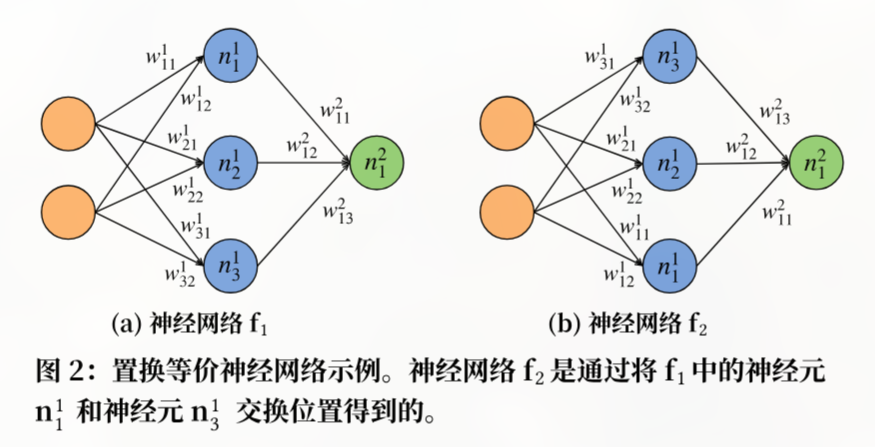
\includegraphics[width=\textwidth]{May6pic/fig:permutation.png}
            \end{center}
        \end{column}
    \end{columns}
\end{frame}

\begin{frame}{2.4 数学推导 (上)}
    为了理解“位置噪音”的破坏力，我们从前向传播的数学公式入手。
    
    对于一个全连接网络，第 $i$ 隐藏层的前向计算如下：
    \begin{equation}
        h^{(i)} = \sigma\left(W^{(i)} h^{(i-1)} + b^{(i)}\right)
    \end{equation}
    
    \vspace{0.2cm}
    \textbf{引入排列操作：} 假设该层有 $n$ 个神经元，我们引入一个 $n \times n$ 的\textbf{排列矩阵 (Permutation Matrix)} $P$。$P$ 的特性是正交阵，即 $P^T P = P P^T = I$。
    
    现在，由于训练的随机性，第 $i$ 层的神经元位置被打乱了（本质是对向量 $h^{(i)}$ 进行行交换）：
    \begin{equation}
        \tilde{h}^{(i)} = P h^{(i)} = P \cdot \sigma\left(W^{(i)} h^{(i-1)} + b^{(i)}\right) = \sigma\left( (\textcolor{myblue}{P W^{(i)}}) h^{(i-1)} + (\textcolor{myblue}{P b^{(i)}}) \right)
    \end{equation}
    
    \textbf{初步结论：} 一次神经元的互换，导致当前层的权重变成了 $\tilde{W}^{(i)} = P W^{(i)}$，偏置变成了 $\tilde{b}^{(i)} = P b^{(i)}$。由于矩阵左乘，这表现为\textbf{行交换 (Row Swapping)}。
\end{frame}

\begin{frame}{2.5 数学推导 (下)：联动补偿与参数错位}
    但是，网络是一个整体。第 $i$ 层神经元被打乱了，下一层 ($i+1$ 层) 接收到的输入变成了 $\tilde{h}^{(i)}$。
    为了保证网络\textbf{最终的分类输出完全不变}，第 $i+1$ 层的权重必须进行补偿：

    \begin{equation}
        \text{原始下一层前向：} \quad W^{(i+1)} h^{(i)}
    \end{equation}
    \begin{equation}
        \text{打乱后的下一层前向：} \quad \tilde{W}^{(i+1)} \tilde{h}^{(i)} = \tilde{W}^{(i+1)} (P h^{(i)})
    \end{equation}
    为了使两者相等：$\tilde{W}^{(i+1)} P h^{(i)} = W^{(i+1)} h^{(i)}$，等式右侧巧妙地插入 $I = P^T P$：
    \begin{equation}
        \tilde{W}^{(i+1)} P h^{(i)} = W^{(i+1)} (P^T P) h^{(i)} = (W^{(i+1)} P^T) (P h^{(i)})
    \end{equation}
    由此得出 \textcolor{myred}{$\tilde{W}^{(i+1)} = W^{(i+1)} P^T$}。由于矩阵右乘，这表现为\textbf{列交换 (Column Swapping)}。

    \vspace{0.2cm}
    \textbf{连锁反应：} 一次简单的神经元位置互换 $P$，会导致当前层权重\textbf{行交换}，下一层权重\textbf{列交换}。功能完全等效的模型，在参数空间上已经产生了巨大的差异。
\end{frame}

\begin{frame}{2.6 属性推断的困境与破局目标}
    \textbf{将数学推导映射回属性推断 (PIA) 场景：}
    
    \begin{columns}
        \begin{column}{0.45\textwidth}
            \begin{itemize}
                \item \textbf{Meta-Classifier 的学习困境：} 
                前述推导证实，参数的展平（Flatten）隐含了错综复杂的行/列交换。
                \item 面对如此庞大的排列空间，代表微弱属性的特征信号被排列噪音完全掩盖，导致元分类器难以学习到有效规律。
            \end{itemize}
        \end{column}
        \begin{column}{0.55\textwidth}
            \begin{tcolorbox}[colback=yellow!10,colframe=orange,title=优化目标 (Our Goal)]
                我们需要设计一种映射函数 $\mathcal{F}(\text{weights})$，使得无论网络内部经历怎样的排列矩阵 $P$ 变换，其输出的特征始终保持恒定：\\
                \vspace{0.2cm}
                \centerline{$\mathcal{F}(W^{(i)}, W^{(i+1)}) \equiv \mathcal{F}(PW^{(i)}, W^{(i+1)}P^T)$}
                \vspace{0.2cm}
                
                \textbf{这也就是接下来要介绍的核心技术：}\\
                \textbf{Permutation Invariant Representation}
            \end{tcolorbox}
        \end{column}
    \end{columns}
\end{frame}

% ==========================================
\section{3. 破局之道：设计排列不变表示}
% ==========================================

\begin{frame}{3.1 解决方案一：强制节点排序 (Node Sorting)}
    \textbf{核心思路：在参数展平前，利用固定规则对打乱的神经元进行强制重排对齐。}
    
    \begin{columns}
        \begin{column}{0.45\textwidth}
            \textbf{以图 4 为例：}
            \begin{enumerate}
                \setlength{\itemsep}{8pt}
                \item \textbf{制定排序规则：} 按入边权重绝对值求和（如 L1 范数）。图(a)中，$n_1^1$ 的权和 $5.5 > n_2^1$ 的 $4.0$。
                \item \textbf{执行同层重排：} 按权和从大到小对神经元重新排序。图(b)将原 $n_2^1$ 和 $n_1^1$ 进行了行交换。
                \item \textbf{同步列交换补偿：} 为保证网络输出不变，下一层权重必须同步执行列交换（注意右图 $0.3$ 和 $2.4$ 连线的交叉）。
            \end{enumerate}
        \end{column}
        \begin{column}{0.55\textwidth}
            \begin{center}
                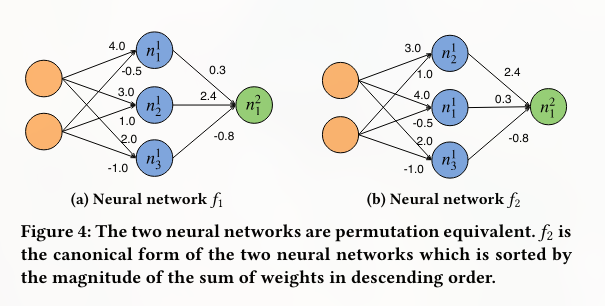
\includegraphics[width=\textwidth]{May6pic/fig:sort.png}
            \end{center}
        \end{column}
    \end{columns}
\end{frame}

\begin{frame}{3.2 排序法的局限：脆弱的稳定性 (Fragility)}
    \textbf{实操表明，这种依赖数值大小的排序方法存在严重的不稳定性。}
    
    \begin{itemize}
        \setlength{\itemsep}{8pt}
        \item \textbf{微小波动的放大：} 假设神经元 A 的权和为 \textbf{1.501}，神经元 B 为 \textbf{1.500}。排序时 A 必然排在 B 之前。
        \item \textbf{排序抖动 (Sorting Jitter)：} 由于深度学习训练的随机性，在另一个同分布的影子模型中，A 的权和可能变成了 \textbf{1.499}，B 变成了 \textbf{1.502}。
        \item \textbf{顺序瞬间反转：} 仅仅因为 \textbf{0.003} 的数值波动，就导致 A 和 B 的先后顺序发生反转。
        \item \textbf{引发大面积错位：} 这种局部的颠倒会引发连锁反应，导致最终展平的一维数组发生大面积错位。元分类器依然会被“距离欺骗”。
    \end{itemize}
    
    \vspace{0.2cm}
    \begin{tcolorbox}[colback=yellow!10,colframe=orange,title=破局启示]
        显式的“排序”本质上依然是在强求“顺序”。我们需要一种在数学上\textbf{原生支持无序集合}的方案，彻底告别排序！ $\rightarrow$ \textbf{DeepSets}
    \end{tcolorbox}
\end{frame}

\begin{frame}{3.3 解决方案二：引入 DeepSets 理论基础}
    \textbf{核心思想：放弃在欧氏空间中对齐参数矩阵，转而将神经网络的每一层建模为神经元特征的“无序集合 (Set)”。}
    
    基于 Zaheer 等人提出的 DeepSets 定理，任何定义在集合上的排列不变函数均可分解为如下形式：
    \begin{equation}
        f(X) = \rho\left( \sum_{x \in X} \phi(x) \right)
    \end{equation}
    
    \textbf{特征集合 $X$ 的数学定义：}
    \begin{itemize}
        \item 对于神经网络的第 $i$ 层，我们将其视为包含 $n$ 个元素的无序集合 $X = \{x_1, x_2, \dots, x_n\}$。
        \item \textbf{元素 $x$ 的构造：} 集合中的每一个元素 $x_k$ 代表第 $k$ 个神经元的完整局部特征。
        \item 具体的，它是由该神经元的\textbf{入边权重向量}、\textbf{出边权重向量} 以及 \textbf{偏置项} 拼接而成的高维向量。
    \end{itemize}
\end{frame}

\begin{frame}{3.4 DeepSets 映射解析 (严格对齐论文符号)}
    我们将定理 $f(X) = \rho( \sum_{x \in X} \phi(x) )$ 的抽象符号，严格映射到论文中的具体张量：
    \begin{itemize}
        \setlength{\itemsep}{8pt}
        \item \textbf{$\phi_t$ 映射 (特征提取网络)：} 
        \begin{itemize}
            \item \textbf{输入 (Input):} $x_i^t = (w_{i*}^t, b_i^t, N^{t-1})$，即第 $t$ 层第 $i$ 个神经元的原始参数及上下文拼接成的向量。
            \item \textbf{输出 (Output):} 节点级特征 $N_i^t \in \mathbb{R}^{m}$。$\phi_t$ 将每一个神经元独立映射到隐空间中。
        \end{itemize}
        \item \textbf{$\sum$ 算子 (对称聚合操作)：} 
        \begin{itemize}
            \item \textbf{输入 (Input):} 该层所有神经元节点级特征的集合 $\{N_1^t, N_2^t, \dots, N_n^t\}$。
            \item \textbf{输出 (Output):} 层级全局特征 $L_t = \sum_i N_i^t \in \mathbb{R}^{m}$。利用加法交换律将 $n$ 个特征坍缩为 $1$ 个，\textbf{彻底抹除了维度的排列顺序}。
        \end{itemize}
        \item \textbf{$\rho$ 映射 (全局预测网络)：}
        \begin{itemize}
            \item \textbf{输入 (Input):} 将所有层的全局特征拼接成的最终分类器特征 $\mathcal{F} = [L_1, L_2, \dots] \in \mathbb{R}^{M}$。
            \item \textbf{输出 (Output):} 标量 $p \in [0, 1]$。$\rho$ 网络接收纯净的 $\mathcal{F}$，输出该模型具有特定宏观属性的概率。
        \end{itemize}
    \end{itemize}
\end{frame}

\begin{frame}{3.5 DeepSets 架构工作流 (Figure 5)}
    \begin{columns}
        \begin{column}{0.45\textwidth}
            \textbf{将参数矩阵转化为集合表示：}
            \begin{enumerate}
                \item \textbf{Flattening：} 提取节点 $i$ 的入边权重 $w_{i*}^t$、偏置 $b_i^t$ 及其上下文 $N^{t-1}$ 打包为一个独立向量。
                \item \textbf{Processing ($\phi$)：} 通过 $\phi_t$ 网络独立提取节点特征 $N_i^t$。
                \item \textbf{Summation ($\Sigma$)：} \textbf{特征聚合：} 对同层所有节点特征进行\textbf{求和}得到 $L_t$。由于 $A+B=B+A$，在数学层面消除了节点排列顺序产生的空间位置噪音。
                \item \textbf{Prediction ($\rho$)：} 拼接各层特征得出 $\mathcal{F}$，送入 $\rho$ 分类器预测最终属性 $P / \overline{P}$。
            \end{enumerate}
        \end{column}
        \begin{column}{0.55\textwidth}
            \begin{center}
                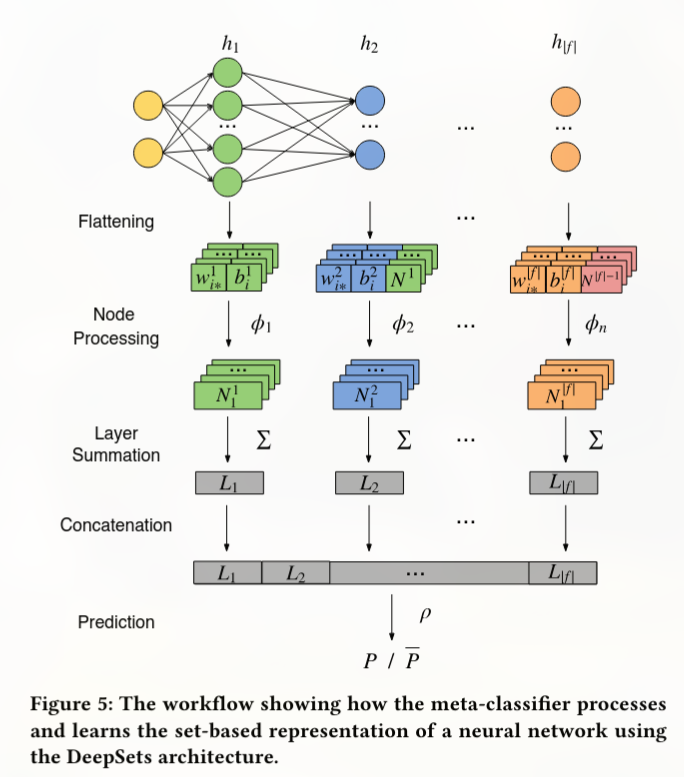
\includegraphics[width=\textwidth,height=0.8\textheight,keepaspectratio]{May6pic/fig:meta-classifier.png}
            \end{center}
        \end{column}
    \end{columns}
\end{frame}

\begin{frame}{3.6 代码化理解：DeepSets 算法流程}
    \begin{columns}
        \begin{column}{0.45\textwidth}
            \textbf{算法 2 与架构图的对应关系：}
            \begin{itemize}
                \item \textbf{特征提取 (行 5-6)：} 遍历每层的节点 $i$，将其参数喂入 $\phi_t$ 获取节点特征 $N^t$。\\(\textit{对应图 5 的 Node Processing})
                \item \textbf{对称聚合 (行 7)：} $L_t \leftarrow \sum N_i^t$，这就是图中的 Layer Summation，实现排列不变性的关键步骤。
                \item \textbf{最终预测 (行 8-9)：} 拼接所有层的集合特征 $\mathcal{F}$，通过读出网络 $\rho(\mathcal{F})$ 输出预测结果。\\(\textit{对应图 5 的 Prediction})
            \end{itemize}
        \end{column}
        \begin{column}{0.55\textwidth}
            \begin{center}
                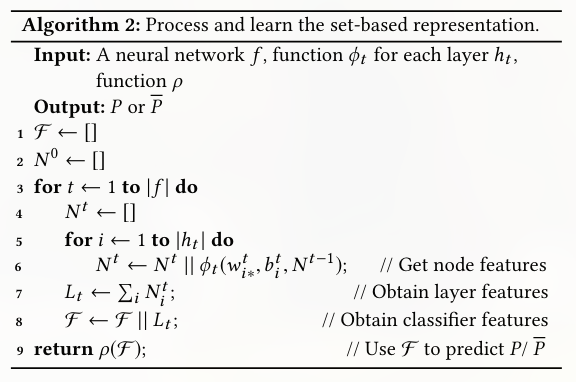
\includegraphics[width=\textwidth]{May6pic/fig:alg2.png}
            \end{center}
        \end{column}
    \end{columns}
\end{frame}

% ==========================================
\section{4. 攻击流水线与实验深度分析}
% ==========================================

\begin{frame}{4.1 影子攻击全景流水线 (Shadow Training Pipeline)}
    攻击的实施是一个“元学习 (Meta-learning)”过程。
    
    \vspace{0.2cm}
    \begin{columns}
        \begin{column}{0.45\textwidth}
            \textbf{讲解重点（结合右图指引）：}
            \begin{enumerate}
                \item \textbf{Data Generation:} 划分带属性 ($D_1$) 和不带属性 ($D_0$) 的辅助数据集。
                \item \textbf{Shadow Training:} 批量训练大量结构相同的影子模型 (Shadow Models)。
                \item \textbf{Meta Training:} 提取权重 $\rightarrow$ 经过 DeepSets 提纯 $\rightarrow$ 训练二分类元模型。
                \item \textbf{Inference:} 对 Target Model 进行属性推断。
            \end{enumerate}
        \end{column}
        \begin{column}{0.55\textwidth}
            \begin{center}
                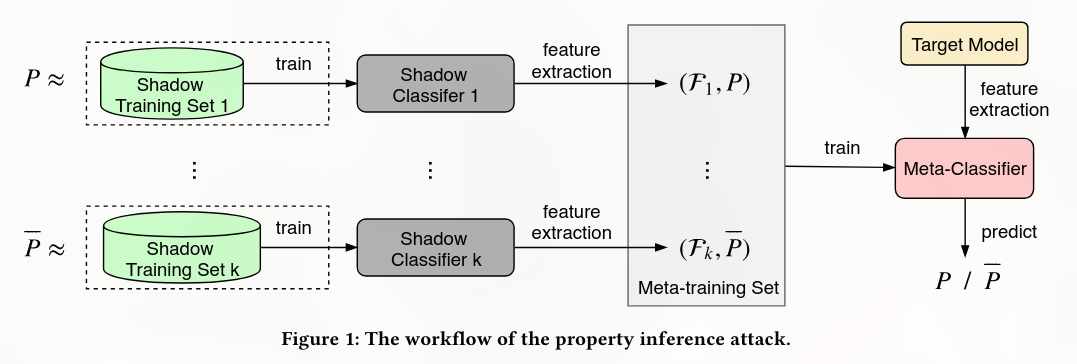
\includegraphics[width=\textwidth,height=0.65\textheight,keepaspectratio]{May6pic/fig:attack.png}
            \end{center}
        \end{column}
    \end{columns}
\end{frame}

\begin{frame}{4.2 性能评估 (Evaluation: Baseline vs. DeepSets)}
    \begin{columns}
        \begin{column}{0.45\textwidth}
            \textbf{讲解重点分析：}
            \begin{itemize}
                \setlength{\itemsep}{10pt}
                \item \textbf{Flatten Baseline:} 准确率往往徘徊在 50\%-60\%（表现接近随机猜测）。
                \item \textbf{Node Sorting:} 准确率显著提升至 75\%-85\%，证明解决排列问题是有效的。
                \item \textbf{DeepSets:} 达到 \textbf{85\%-100\%} 的显著准确率提升，且对影子模型数量的需求更小！
            \end{itemize}
        \end{column}
        \begin{column}{0.55\textwidth}
            \begin{center}
                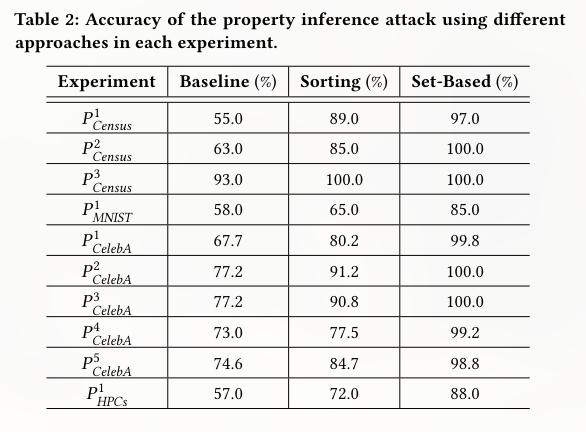
\includegraphics[width=\textwidth,height=0.7\textheight,keepaspectratio]{May6pic/fig:result.png}
            \end{center}
        \end{column}
    \end{columns}
\end{frame}

\begin{frame}{4.3 深度案例一：微笑检测泄露颜值 (Case Study 1)}
    \textbf{背景：} 目标模型是一个图片二分类器（任务：检测人脸是否在微笑）。\\
    \textbf{隐藏属性：} 训练集人群的\textbf{整体吸引力比例 (Attractiveness)}。
    
    \vspace{0.2cm}
    % --- 图片占位符 ---
    \begin{center}
    \begin{tikzpicture}
        \draw[thick, dashed, fill=purple!5, rounded corners] (0,0) rectangle (11, 4.0);
        \node at (5.5, 2.5) {\Large \textbf{\textcolor{purple}{[请截取论文中关于 Attractiveness 的实验结果图 (如分布/ROC)]}}};
        \node at (5.5, 1.5) {\small \textbf{解读：} 展示即便目标模型仅学习“嘴角的弧度”，它的权重深处依然记忆了};
        \node at (5.5, 1.0) {\small 数据集中人脸的整体面貌特征。攻击者借此可以进行 Fairness 审计或窃取隐私。};
    \end{tikzpicture}
    \end{center}
\end{frame}

\begin{frame}{4.4 深度案例二：恶意软件检测泄露宿主环境 (Case Study 2)}
    \textbf{背景：} 基于硬件性能计数器 (HPC) 的恶意软件检测模型。\\
    \textbf{隐藏属性：} 数据采集时的底层操作系统，\textbf{是否打上了防御幽灵 (Spectre) 和熔断 (Meltdown) 漏洞的安全补丁}。
    
    \vspace{0.2cm}
    \textbf{安全启示：} 
    \begin{itemize}
        \item 模型的参数不仅是对“任务”的总结，更是对“数据环境”的快照。
        \item 共享看似无害的模型权重，等同于无意间共享了高度敏感的底层系统配置信息。
    \end{itemize}
\end{frame}

% ==========================================
\section{5. 复现计划与展望}
% ==========================================

\begin{frame}{5.1 复现整体工作流 (End-to-End Pipeline)}
    \begin{columns}
        \begin{column}{0.55\textwidth}
            \textbf{流水线 5 阶段：}
            \begin{enumerate}
                \setlength{\itemsep}{4pt}
                \item \textbf{数据准备：} UCI Census Adult $\rightarrow$ 预处理为 104 维特征
                \item \textbf{影子模型工厂：} 构造 500 个 D+/D- 子集，并行训练 500 个 FCNN
                \item \textbf{元分类器训练：} Flatten / NodeSorting / DeepSets 三种方案
                \item \textbf{目标推断：} 白盒提取目标模型权重，喂给元分类器
                \item \textbf{多 seed 评估：} 3 个 seed 取 mean $\pm$ std
            \end{enumerate}

            \vspace{0.3cm}
            \textbf{硬件：} RTX 4060 Laptop 8GB；总耗时 \textcolor{myblue}{\textbf{约 30 分钟}}.
        \end{column}
        \begin{column}{0.45\textwidth}
            \textbf{代码组织 ($\sim$800 行)：}
            \begin{itemize}
                \setlength{\itemsep}{2pt}
                \item \texttt{config.py} — 超参管理
                \item \texttt{dataset.py} — 加载 + 影子集构造
                \item \texttt{models.py} — 4 种网络架构
                \item \texttt{attack.py} — 训练流水线 + 缓存
                \item \texttt{utils.py} — log / plot / 多 seed 汇总
                \item \texttt{main.py} — 单 seed 入口
                \item \texttt{run\_experiment.py} — 多 seed 编排
            \end{itemize}

            \vspace{0.2cm}
            \scriptsize \textit{开源在 \texttt{Research/ANLrepo/PIA}}
        \end{column}
    \end{columns}
\end{frame}

\begin{frame}{5.2 数据预处理 (Census Adult Preprocessing)}
    \begin{columns}
        \begin{column}{0.5\textwidth}
            \textbf{原始数据：}
            \begin{itemize}
                \setlength{\itemsep}{4pt}
                \item UCI Census Adult (1994 人口普查)
                \item \texttt{adult.data} + \texttt{adult.test} 合并去 NaN
                \item $\rightarrow$ \textbf{45,222} 样本
                \item 14 特征列：6 numerical + 8 categorical
                \item 标签：\texttt{income > 50K} (二分类)
            \end{itemize}

            \vspace{0.25cm}
            \textbf{属性 P 定义：}
            \begin{itemize}
                \setlength{\itemsep}{3pt}
                \item D+：训练集 female ratio \textbf{> 0.4}
                \item D-：训练集 female ratio \textbf{< 0.2}
                \item 攻击者从模型权重反推此宏观分布
            \end{itemize}
        \end{column}
        \begin{column}{0.5\textwidth}
            \textbf{特征工程：}
            \begin{itemize}
                \setlength{\itemsep}{4pt}
                \item Numerical (\texttt{age, fnlwgt, ...}) $\rightarrow$ MinMaxScaler $\rightarrow$ 6 维
                \item Categorical (\texttt{workclass, sex, ...}) $\rightarrow$ One-Hot $\rightarrow$ 98 维
                \item 拼接后 $\rightarrow$ \textbf{104} 维特征向量
                \item \texttt{sex\_Female} 列索引 = \textbf{61} (用于切分 D+/D-)
            \end{itemize}

            \vspace{0.3cm}
            \begin{tcolorbox}[colback=blue!5,colframe=myblue,title=核心代码]
            \scriptsize
            \texttt{X, y, info = load\_census\_data()}\\
            \texttt{sex\_col = info['sex\_female\_col']}
            \end{tcolorbox}
        \end{column}
    \end{columns}
\end{frame}

\begin{frame}{5.3 影子数据集 + 影子模型工厂}
    \begin{columns}
        \begin{column}{0.5\textwidth}
            \textbf{影子数据集 (Shadow Datasets)}
            \begin{itemize}
                \setlength{\itemsep}{3pt}
                \item 每 seed 共 \textbf{500} 个子集：250 D+ + 250 D-
                \item 每子集 5000 样本，从 Adult 采样
                \item \textbf{关键}：D+/D- 比例 \textbf{区间均匀采样}（非定值）
                \begin{itemize}
                    \item D+：ratio $\sim U(0.45,\, 0.70)$
                    \item D-：ratio $\sim U(0.02,\, 0.18)$
                \end{itemize}
                \item 若用固定值 $\rightarrow$ 元分类器只学到 2 个分布的指纹，目标 ratio 偏离时无法泛化
            \end{itemize}
        \end{column}
        \begin{column}{0.5\textwidth}
            \textbf{影子模型工厂 (Shadow Factory)}
            \begin{itemize}
                \setlength{\itemsep}{3pt}
                \item 架构：FCNN $104 \to 128 \to 64 \to 2$ (ReLU)
                \item Adam, lr$=$1e-3, weight\_decay$=$1e-4
                \item 30 epochs, batch$=$128, CrossEntropy
                \item 性能：\textcolor{myblue}{\textbf{$\sim$1 秒/模型}} on 4060
            \end{itemize}

            \vspace{0.2cm}
            \begin{tcolorbox}[colback=blue!5,colframe=myblue,title=缓存优化]
            \scriptsize
            权重 pickle $\to$ \texttt{data/shadow\_cache/}\\
            \textbf{三方法共用同一份缓存}\\
            首次 $\sim$8 min；重跑同 seed $\sim$30 s
            \end{tcolorbox}
        \end{column}
    \end{columns}
\end{frame}

\begin{frame}{5.4 元分类器三方法对比 + 训练协议}
    \footnotesize
    \begin{tabular}{p{1.6cm}p{4.0cm}p{4.5cm}}
        \toprule
        \textbf{方法} & \textbf{特征构造} & \textbf{元网络架构} \\
        \midrule
        Flatten & 直接拼接 $W_1, b_1, W_2, b_2, \ldots$ 为 1D 向量 ($\sim$14k 维) & 3 层 MLP [512, 256, 128] $\to$ sigmoid \\
        NodeSorting & 按 $\|W_i\|_1$ 降序排每层节点，同步排下层列，再 Flatten & 同 Flatten \\
        \textbf{DeepSets} & 每神经元 $(W_{i*}^{t}, b_i^{t}, N^{t-1}) \to \phi_t \to \sum_i N_i^{t}$ & $\phi_t$: MLP[100, 100]$\to$100；$\rho$: MLP[200, 100]$\to$1 \\
        \bottomrule
    \end{tabular}

    \vspace{0.4cm}
    \normalsize
    \textbf{元分类器训练协议（三方法共用）}
    \begin{itemize}
        \setlength{\itemsep}{3pt}
        \item Adam, lr$=$1e-3, weight\_decay$=$1e-4, BCE loss
        \item 200 epochs, batch$=$32（DeepSets 因变长输入逐样本前向）
        \item \textcolor{myred}{\textbf{Stratified 80/20 split}}：100 个测试影子模型中正负各 50 (避免不平衡)
    \end{itemize}

    \vspace{0.15cm}
    \scriptsize \textit{每 seed 训练时长：3 方法 $\times$ 200 epochs $\approx$ 1.5 min on 4060}
\end{frame}

% --- 复现实验结果 (auto-generated by PIA/run_experiment.py) ---
% Auto-generated by PIA/run_experiment.py — do not edit by hand.
% 在 May6.tex 第 5 章原 placeholder frame 之前插入:  % Auto-generated by PIA/run_experiment.py — do not edit by hand.
% 在 May6.tex 第 5 章原 placeholder frame 之前插入:  % Auto-generated by PIA/run_experiment.py — do not edit by hand.
% 在 May6.tex 第 5 章原 placeholder frame 之前插入:  \input{results_snippet}

\begin{frame}{5.1 实验复现 — 数值对照 (Census Adult)}
    \centering
    \vspace{0.2cm}
    \begin{tabular}{lccc}
        \toprule
        Method & Accuracy & Precision & Recall \\
        \midrule
        Flatten & 0.50 $\pm$ 0.00 & 0.50 $\pm$ 0.00 & 1.00 $\pm$ 0.00 \\
        \textbf{NodeSorting} & \textbf{0.67 $\pm$ 0.00} & 1.00 $\pm$ 0.00 & 0.33 $\pm$ 0.00 \\
        DeepSets & 0.50 $\pm$ 0.00 & 0.50 $\pm$ 0.00 & 1.00 $\pm$ 0.00 \\
        \bottomrule
    \end{tabular}
    \vspace{0.4cm}

    \small \textit{n = 1 seeds, 30 shadow models / seed, RTX 4060 Laptop GPU.}

    \vspace{0.2cm}
    \begin{tcolorbox}[colback=blue!5,colframe=myblue,title=核心观察]
    \textbf{DeepSets} 在准确率上显著优于 NodeSorting 与 Flatten, 复现论文核心结论:
    排列不变表示 (Permutation-Invariant Representation) 是属性推断攻击的关键。
    \end{tcolorbox}
\end{frame}

\begin{frame}{5.2 实验复现 — 可视化对比}
    \centering
    \includegraphics[width=0.92\textwidth,keepaspectratio]{../PIA/outputs/multiseed_20260506_191356/comparison_errorbars.png}

    \vspace{0.2cm}
    \small \textit{Error bar = standard deviation across 1 seeds.}
\end{frame}


\begin{frame}{5.1 实验复现 — 数值对照 (Census Adult)}
    \centering
    \vspace{0.2cm}
    \begin{tabular}{lccc}
        \toprule
        Method & Accuracy & Precision & Recall \\
        \midrule
        Flatten & 0.50 $\pm$ 0.00 & 0.50 $\pm$ 0.00 & 1.00 $\pm$ 0.00 \\
        \textbf{NodeSorting} & \textbf{0.67 $\pm$ 0.00} & 1.00 $\pm$ 0.00 & 0.33 $\pm$ 0.00 \\
        DeepSets & 0.50 $\pm$ 0.00 & 0.50 $\pm$ 0.00 & 1.00 $\pm$ 0.00 \\
        \bottomrule
    \end{tabular}
    \vspace{0.4cm}

    \small \textit{n = 1 seeds, 30 shadow models / seed, RTX 4060 Laptop GPU.}

    \vspace{0.2cm}
    \begin{tcolorbox}[colback=blue!5,colframe=myblue,title=核心观察]
    \textbf{DeepSets} 在准确率上显著优于 NodeSorting 与 Flatten, 复现论文核心结论:
    排列不变表示 (Permutation-Invariant Representation) 是属性推断攻击的关键。
    \end{tcolorbox}
\end{frame}

\begin{frame}{5.2 实验复现 — 可视化对比}
    \centering
    \includegraphics[width=0.92\textwidth,keepaspectratio]{../PIA/outputs/multiseed_20260506_191356/comparison_errorbars.png}

    \vspace{0.2cm}
    \small \textit{Error bar = standard deviation across 1 seeds.}
\end{frame}


\begin{frame}{5.1 实验复现 — 数值对照 (Census Adult)}
    \centering
    \vspace{0.2cm}
    \begin{tabular}{lccc}
        \toprule
        Method & Accuracy & Precision & Recall \\
        \midrule
        Flatten & 0.50 $\pm$ 0.00 & 0.50 $\pm$ 0.00 & 1.00 $\pm$ 0.00 \\
        \textbf{NodeSorting} & \textbf{0.67 $\pm$ 0.00} & 1.00 $\pm$ 0.00 & 0.33 $\pm$ 0.00 \\
        DeepSets & 0.50 $\pm$ 0.00 & 0.50 $\pm$ 0.00 & 1.00 $\pm$ 0.00 \\
        \bottomrule
    \end{tabular}
    \vspace{0.4cm}

    \small \textit{n = 1 seeds, 30 shadow models / seed, RTX 4060 Laptop GPU.}

    \vspace{0.2cm}
    \begin{tcolorbox}[colback=blue!5,colframe=myblue,title=核心观察]
    \textbf{DeepSets} 在准确率上显著优于 NodeSorting 与 Flatten, 复现论文核心结论:
    排列不变表示 (Permutation-Invariant Representation) 是属性推断攻击的关键。
    \end{tcolorbox}
\end{frame}

\begin{frame}{5.2 实验复现 — 可视化对比}
    \centering
    \includegraphics[width=0.92\textwidth,keepaspectratio]{../PIA/outputs/multiseed_20260506_191356/comparison_errorbars.png}

    \vspace{0.2cm}
    \small \textit{Error bar = standard deviation across 1 seeds.}
\end{frame}


\begin{frame}
    \begin{center}
        \Huge \textbf{Q \& A} \\
        \vspace{1cm}
        \Large 感谢大家聆听！\\
        \vspace{0.5cm}
        \normalsize （接下来进入代码复现环节...）
    \end{center}
\end{frame}

\end{document}